\documentclass[border=10pt]{standalone}
\usepackage[svgnames]{xcolor}
\usepackage{amsmath}
\usepackage{pgfplots}
\pgfplotsset{compat=newest}
\usepackage[sfdefault]{FiraSans}
\usepackage{FiraMono}
\renewcommand*\familydefault{\sfdefault}
\begin{document}
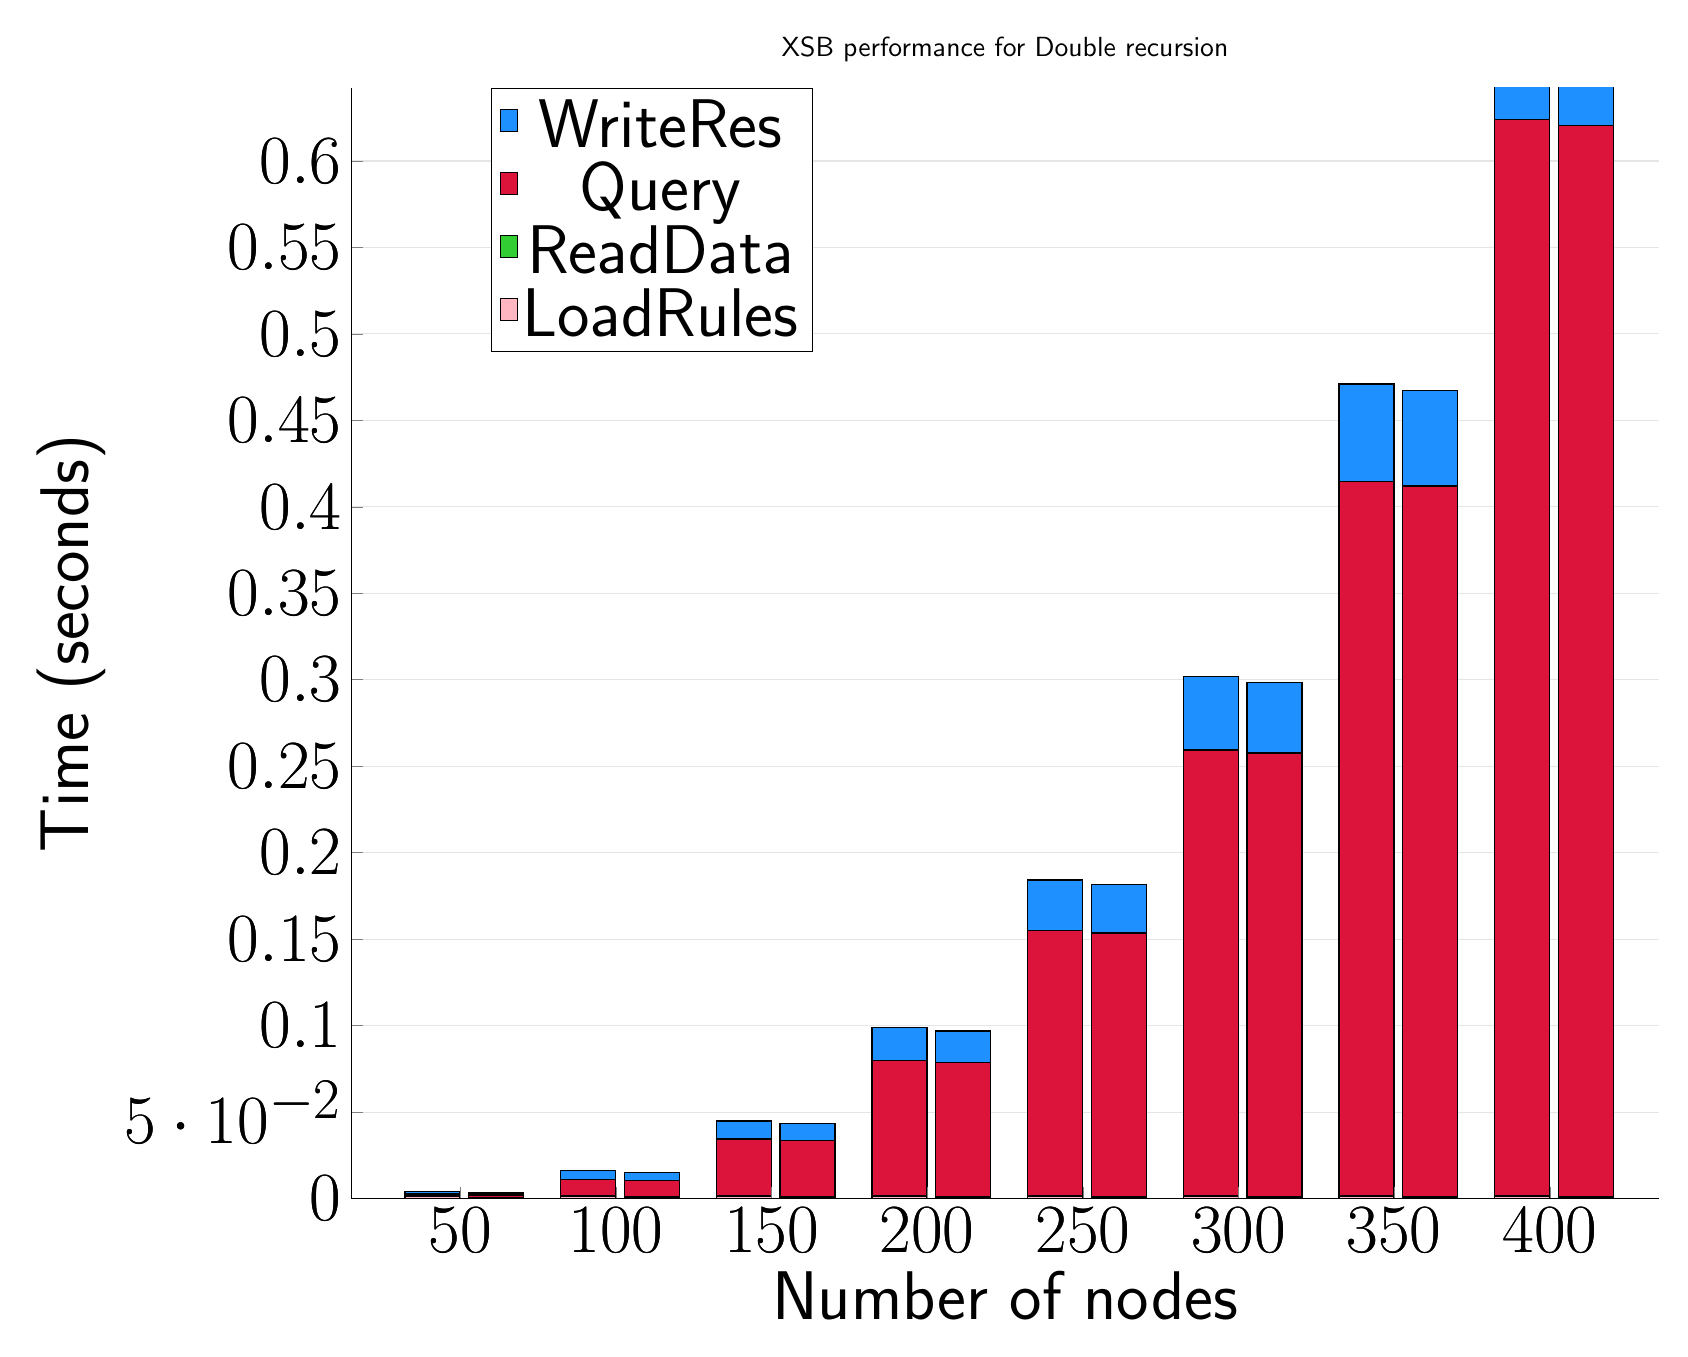
\begin{tikzpicture}
	\begin{axis}[
			ybar stacked,
			title={XSB performance for Double recursion},
			bar shift=-10pt,
			width=1.5\textwidth,
			bar width=0.7cm,
			ymajorgrids, tick align=inside,
			major grid style={draw=gray!20},
			xtick=data,
			ymin=0, ymax=0.6422704648971556,
			axis x line*=bottom,
			axis y line*=left,
			enlarge x limits=0.1,
			legend style={
					at={(0.23, 1)},
					anchor=north,
					legend columns=1,
					font=\Huge,
				},
			ylabel={Time (seconds)},
			xlabel={Number of nodes},
			label style={font=\Huge},
			tick label style={font=\Huge},
		]
		\addlegendimage{fill=DodgerBlue, draw=black, line width=0.2pt}
		\addlegendentry{WriteRes}
		\addlegendimage{fill=Crimson, draw=black, line width=0.2pt}
		\addlegendentry{Query}
		\addlegendimage{fill=LimeGreen, draw=black, line width=0.2pt}
		\addlegendentry{ReadData}
		\addlegendimage{fill=LightPink, draw=black, line width=0.2pt}
		\addlegendentry{LoadRules}
		\addplot +[fill=LightPink, draw=black, line width=0.5pt] coordinates {
				(50, 0.001029872894287108)
				(100, 0.001071524620056153)
				(150, 0.001039052009582521)
				(200, 0.001047062873840331)
				(250, 0.0010452508926391602)
				(300, 0.001081418991088866)
				(350, 0.0010599613189697268)
				(400, 0.001096749305725099)
			};
		\addplot +[fill=LimeGreen, draw=black, line width=0.5pt] coordinates {
				(50, 0.0003611326217651368)
				(100, 0.00040781497955322276)
				(150, 0.00045676231384277326)
				(200, 0.0005148410797119142)
				(250, 0.0005582332611083985)
				(300, 0.0006087541580200197)
				(350, 0.0006557226181030274)
				(400, 0.0007033824920654296)
			};
		\addplot +[fill=Crimson, draw=black, line width=0.5pt] coordinates {
				(50, 0.001232457160949707)
				(100, 0.009635353088378904)
				(150, 0.03290550708770753)
				(200, 0.07824118137359619)
				(250, 0.1535104036331178)
				(300, 0.2577409267425537)
				(350, 0.4129061460494995)
				(400, 0.6222704648971555)
			};
		\addplot +[fill=DodgerBlue, draw=black, line width=0.5pt] coordinates {
				(50, 0.001361703872680664)
				(100, 0.0049999952316284344)
				(150, 0.01035854816436766)
				(200, 0.01929423809051515)
				(250, 0.0290255069732665)
				(300, 0.0424486637115479)
				(350, 0.056340050697326685)
				(400, 0.07606353759765658)
			};
	\end{axis}
	\begin{axis}[
			ybar stacked,
			bar shift=13pt,
			width=1.5\textwidth,
			bar width=0.7cm,
			ymajorgrids, tick align=inside,
			major grid style={draw=none},
			xtick=data,
			ymin=0, ymax=0.6422704648971556,
			axis x line*=none,
			axis y line*=none,
			enlarge x limits=0.1,
			label style={font=\Huge},
			tick label style={font=\Huge},
		]
		\addplot +[fill=LightPink, draw=black, line width=0.5pt] coordinates {
				(50, 0.0005971999999999998)
				(100, 0.0006169999999999998)
				(150, 0.0005948000000000001)
				(200, 0.0006047000000000003)
				(250, 0.0006054000000000003)
				(300, 0.0006120000000000003)
				(350, 0.0006151000000000002)
				(400, 0.0006180000000000001)
			};
		\addplot +[fill=LimeGreen, draw=black, line width=0.5pt] coordinates {
				(50, 0.0001718)
				(100, 0.0002208)
				(150, 0.0002559000000000001)
				(200, 0.00030809999999999985)
				(250, 0.00034659999999999997)
				(300, 0.00039219999999999994)
				(350, 0.00043989999999999947)
				(400, 0.0004864999999999994)
			};
		\addplot +[fill=Crimson, draw=black, line width=0.5pt] coordinates {
				(50, 0.0012109999999999998)
				(100, 0.0095396)
				(150, 0.03263)
				(200, 0.07761490000000001)
				(250, 0.15253049999999999)
				(300, 0.25664099999999995)
				(350, 0.4110653)
				(400, 0.6193593000000001)
			};
		\addplot +[fill=DodgerBlue, draw=black, line width=0.5pt] coordinates {
				(50, 0.0011376)
				(100, 0.004636500000000002)
				(150, 0.009911)
				(200, 0.018389199999999998)
				(250, 0.028097499999999997)
				(300, 0.04093370000000001)
				(350, 0.055071400000000006)
				(400, 0.0723582)
			};
	\end{axis}
\end{tikzpicture}

\end{document}
